\documentclass[11pt, a4paper]{article}
\usepackage{pdfpages}
\usepackage{parallel}
\usepackage[T2A]{fontenc}
%\usepackage{ucs}
\usepackage[utf8]{inputenc}
\usepackage[english,russian]{babel}
\usepackage{hyperref}
\usepackage{rotating}
\usepackage[inner=2cm,top=1.8cm,outer=2cm,bottom=2.3cm,nohead]{geometry}
%\usepackage{listings}
\usepackage{graphicx}
\usepackage{wrapfig}
\usepackage{longtable}
\usepackage{indentfirst}
\usepackage{array}
\usepackage{tikzsymbols}
\usepackage{soul}
\usepackage[ruled,vlined]{algorithm2e}
\usepackage{qrcode}
\counterwithout{figure}{section} 

\usepackage{url}
\makeatletter
\g@addto@macro{\UrlBreaks}{\UrlOrds}
\makeatother

\newcolumntype{P}[1]{>{\raggedright\arraybackslash}p{#1}}
\frenchspacing
%\usepackage{fixltx2e} %text sub- and superscripts
\usepackage{icomma} % коскі ў матэматычным рэжыме
%\PreloadUnicodePage{4}

\newcommand{\longpage}{\enlargethispage{\baselineskip}}
\newcommand{\shortpage}{\enlargethispage{-\baselineskip}}

\def\switchlang#1{\expandafter\csname switchlang#1\endcsname}
\def\switchlangbe{
\let\saverefname=\refname%
\def\refname{Літаратура}%
\def\figurename{Іл.}%
}
\def\switchlangru{
\let\saverefname=\refname%
\let\savefigurename=\figurename%
\def\refname{Литература}%
\def\figurename{Рис.}%
}
\def\switchlangen{
\let\saverefname=\refname%
\def\refname{References}%
\def\figurename{Fig.}%
}

\hyphenation{admi-ni-stra-tive}
\hyphenation{ex-pe-ri-ence}
\hyphenation{fle-xi-bi-li-ty}
\hyphenation{Py-thon}
\hyphenation{ma-the-ma-ti-cal}
\hyphenation{re-ported}
\hyphenation{imp-le-menta-tions}
\hyphenation{pro-vides}
\hyphenation{en-gi-neering}
\hyphenation{com-pa-ti-bi-li-ty}
\hyphenation{im-pos-sible}
\hyphenation{desk-top}
\hyphenation{elec-tro-nic}
\hyphenation{com-pa-ny}
\hyphenation{de-ve-lop-ment}
\hyphenation{de-ve-loping}
\hyphenation{de-ve-lop}
\hyphenation{da-ta-ba-se}
\hyphenation{plat-forms}
\hyphenation{or-ga-ni-za-tion}
\hyphenation{pro-gramming}
\hyphenation{in-stru-ments}
\hyphenation{Li-nux}
\hyphenation{sour-ce}
\hyphenation{en-vi-ron-ment}
\hyphenation{Te-le-pathy}
\hyphenation{Li-nux-ov-ka}
\hyphenation{Open-BSD}
\hyphenation{Free-BSD}
\hyphenation{men-ti-on-ed}
\hyphenation{app-li-ca-tion}

\def\progref!#1!{\texttt{#1}}
\renewcommand{\arraystretch}{2} %Іначай формулы ў матрыцы зліпаюцца з лініямі
\usepackage{array}

\def\interview #1 (#2), #3, #4, #5\par{

\section[#1, #3, #4]{#1 -- #3, #4}
\def\qname{LVEE}
\def\aname{#1}
\def\q ##1\par{{\noindent \bf \qname: ##1 }\par}
\def\a{{\noindent \bf \aname: } \def\qname{L}\def\aname{#2}}
}

\def\interview* #1 (#2), #3, #4, #5\par{

\section*{#1\\{\small\rm #3, #4. #5}}
\ifx\ParallelWhichBox\undefined%
    \addcontentsline{toc}{section}{#1, #3, #4}%
\else%
\ifnum\ParallelWhichBox=0%
    \addcontentsline{toc}{section}{#1, #3, #4}%
\fi\fi%

\def\qname{LVEE}
\def\aname{#1}
\def\q ##1\par{{\noindent \bf \qname: ##1 }\par}
\def\a{{\noindent \bf \aname: } \def\qname{L}\def\aname{#2}}
}

\newcommand{\interviewfooter}[1]{
\vskip 1em
\noindent \textit{#1}
}

\AtEndDocument{\vfill\centering \qrcode{https://github.com/fiowro/mouses/blob/main/\jobname.pdf}}

\switchlang{ru}
\begin{document}

\title{1975 "--- Tektronix 4952 joystick}
\date{}
\maketitle
\selectlanguage{russian}

Джойстик Tektronix 4952 (рис. \ref{fig:TektronixJoystickPic}) был разработан для текстовых и графических компьютерных терминалов серии 4010 и аналогичных настольных компьютеров серии 4050 на основе технологии запоминающих электронно-лучевых трубок, созданной Tektronix, чтобы обеспечивать высокое разрешение экрана (до 1024x780) без использования видеопамяти \cite{wiki}. Такие устройства производились Tektronix в конце 1970-х — начале 1980-х годов, до появиления более дешевых рабочих станций UNIX. О пополнении линейки периферийных устройств джойстиком было объявлено в 1974 году \cite{adv}, но известные экземпляры документации датируются следующим годом.

\begin{figure}[h]
   \centering
    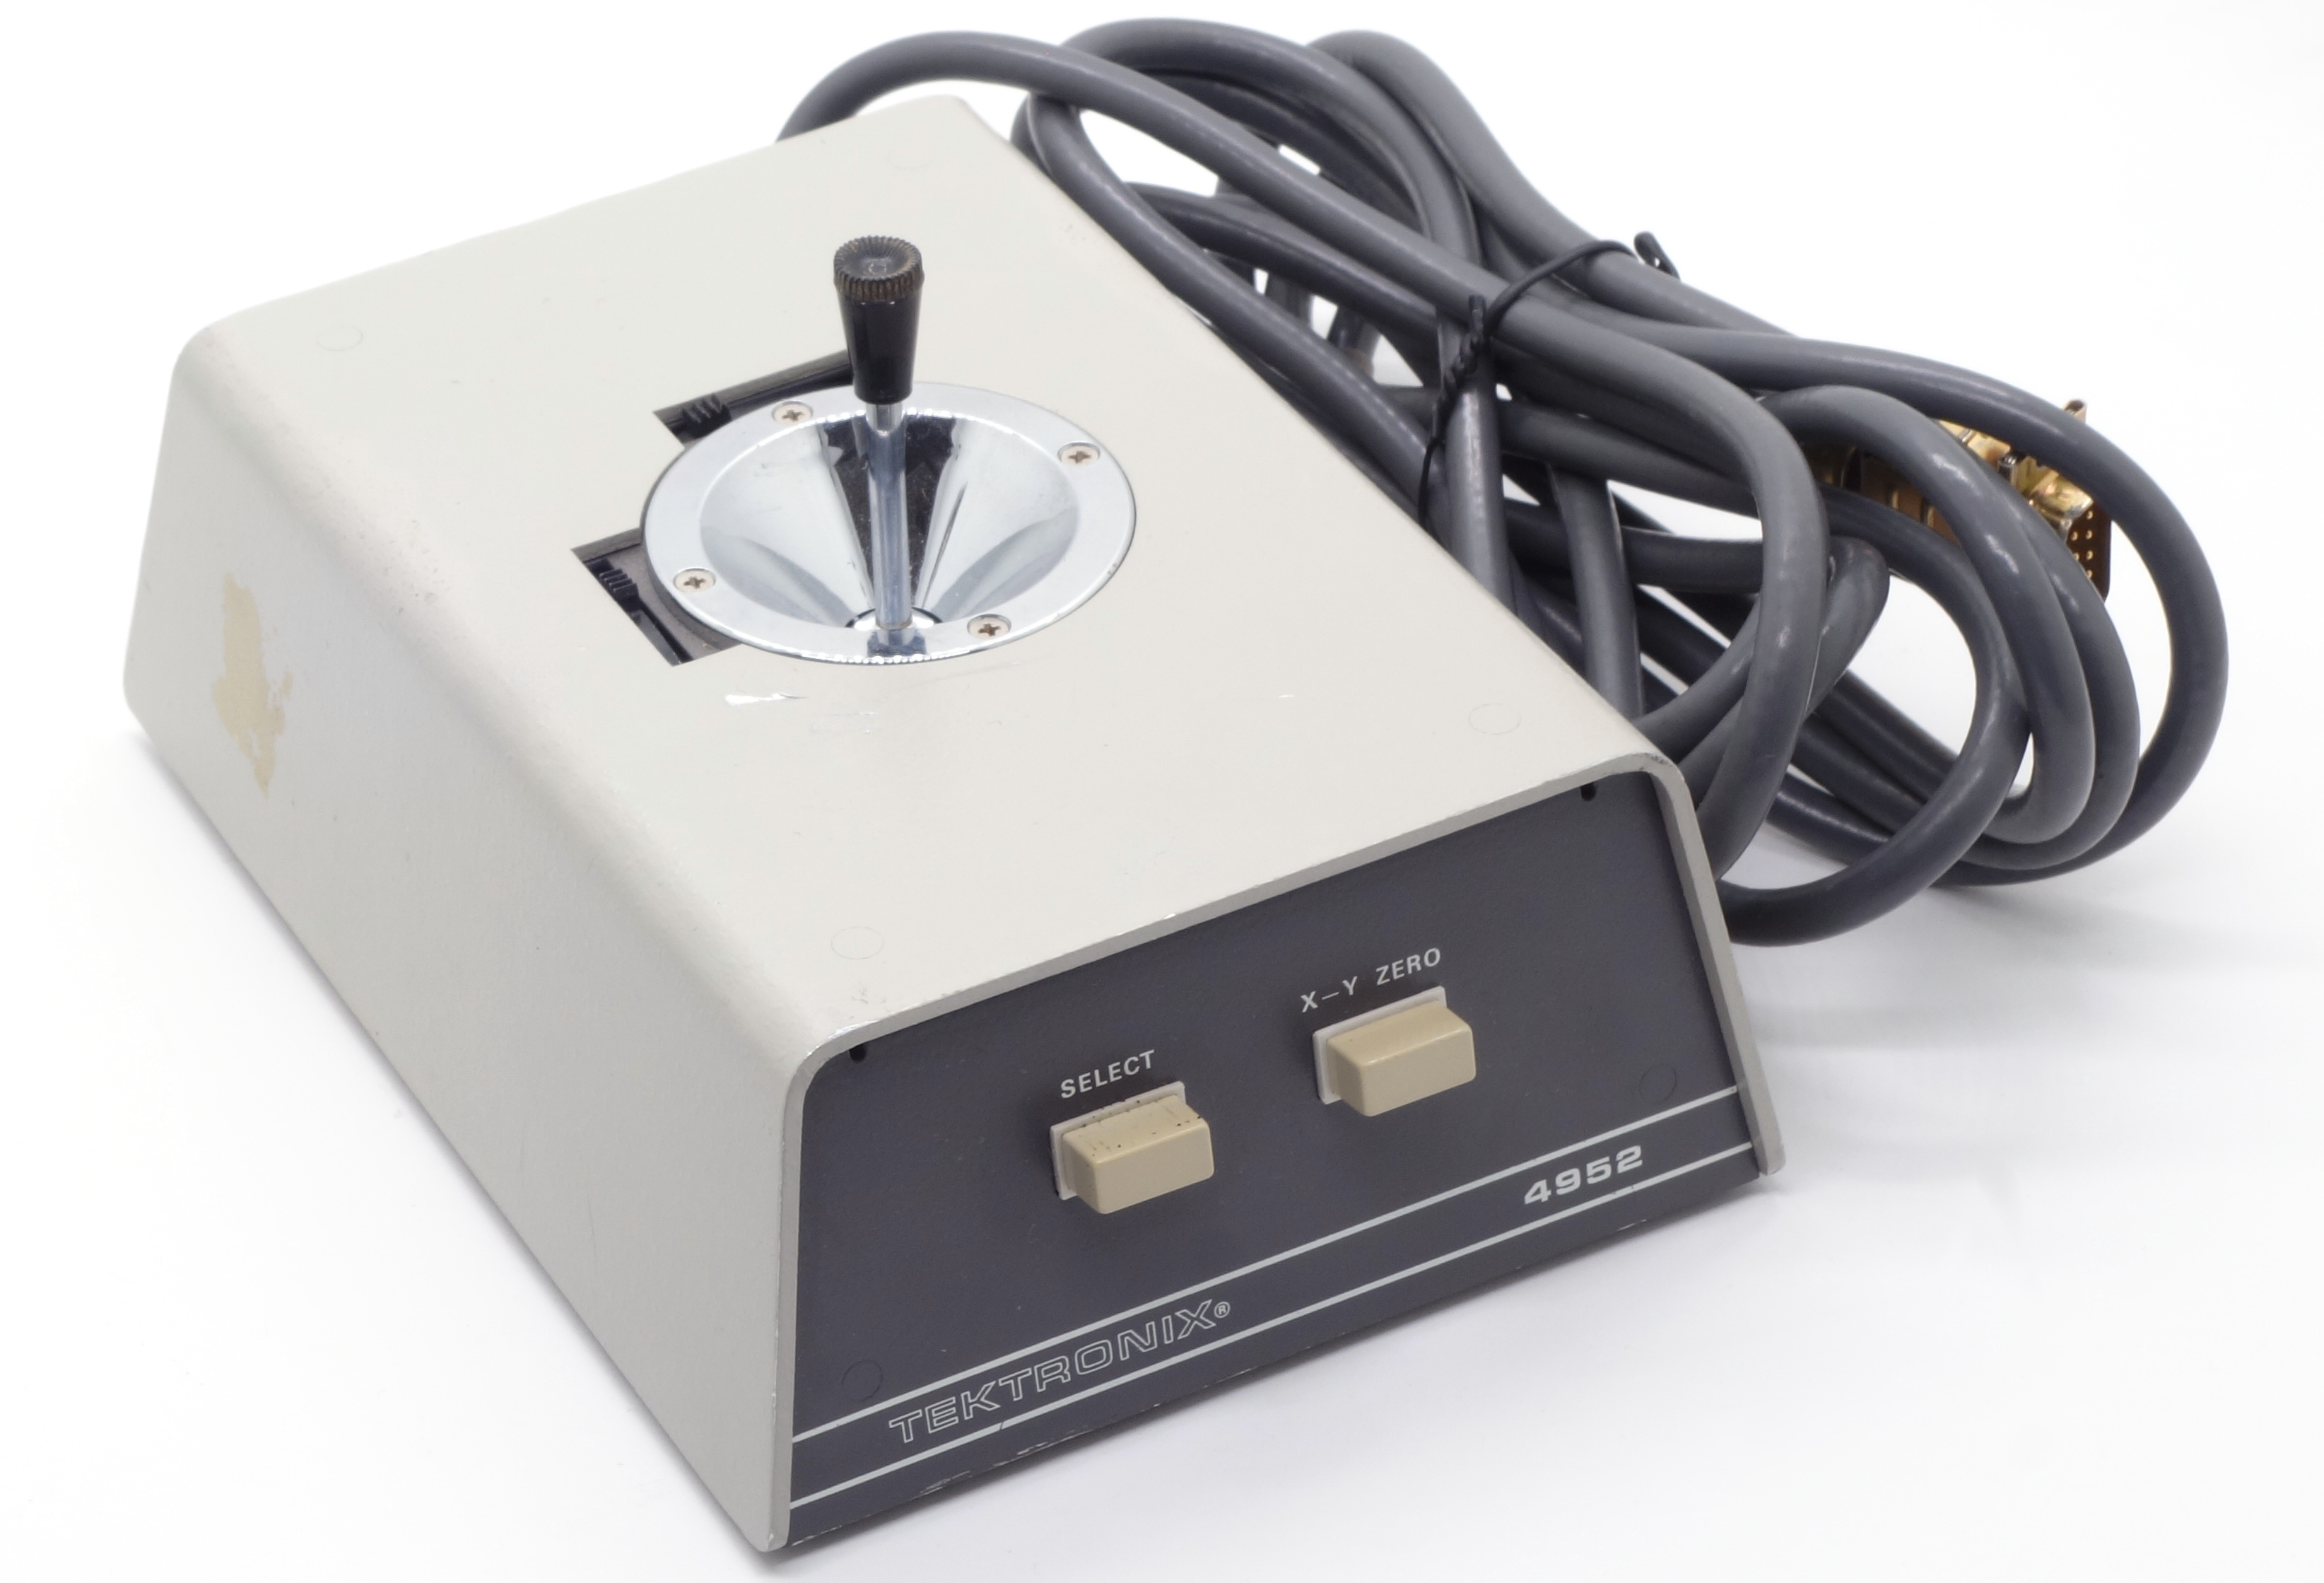
\includegraphics[scale=0.45]{1975_Tektronix_4952_Joystick/pic_30.jpg}
    \caption{Джойстик Tektronix 4952}
    \label{fig:TektronixJoystickPic}
\end{figure}

Джойстик имеет резиновые ножки и металлический корпус. На верхней стороне (рис. \ref{fig:TektronixJoystickTopAndBottom}) находятся два триммера \cite{manual} и небольшая рукоятка («рычаг управления» или «control lever» в терминологии производителя). Внешний вид соответствует терминалам и компьютерам Tektronix "--- моноблокам с дисплеем, клавиатурой, процессором и стримером в общем напольном корпусе \cite{wiki}.

\begin{figure}[h]
    \centering
    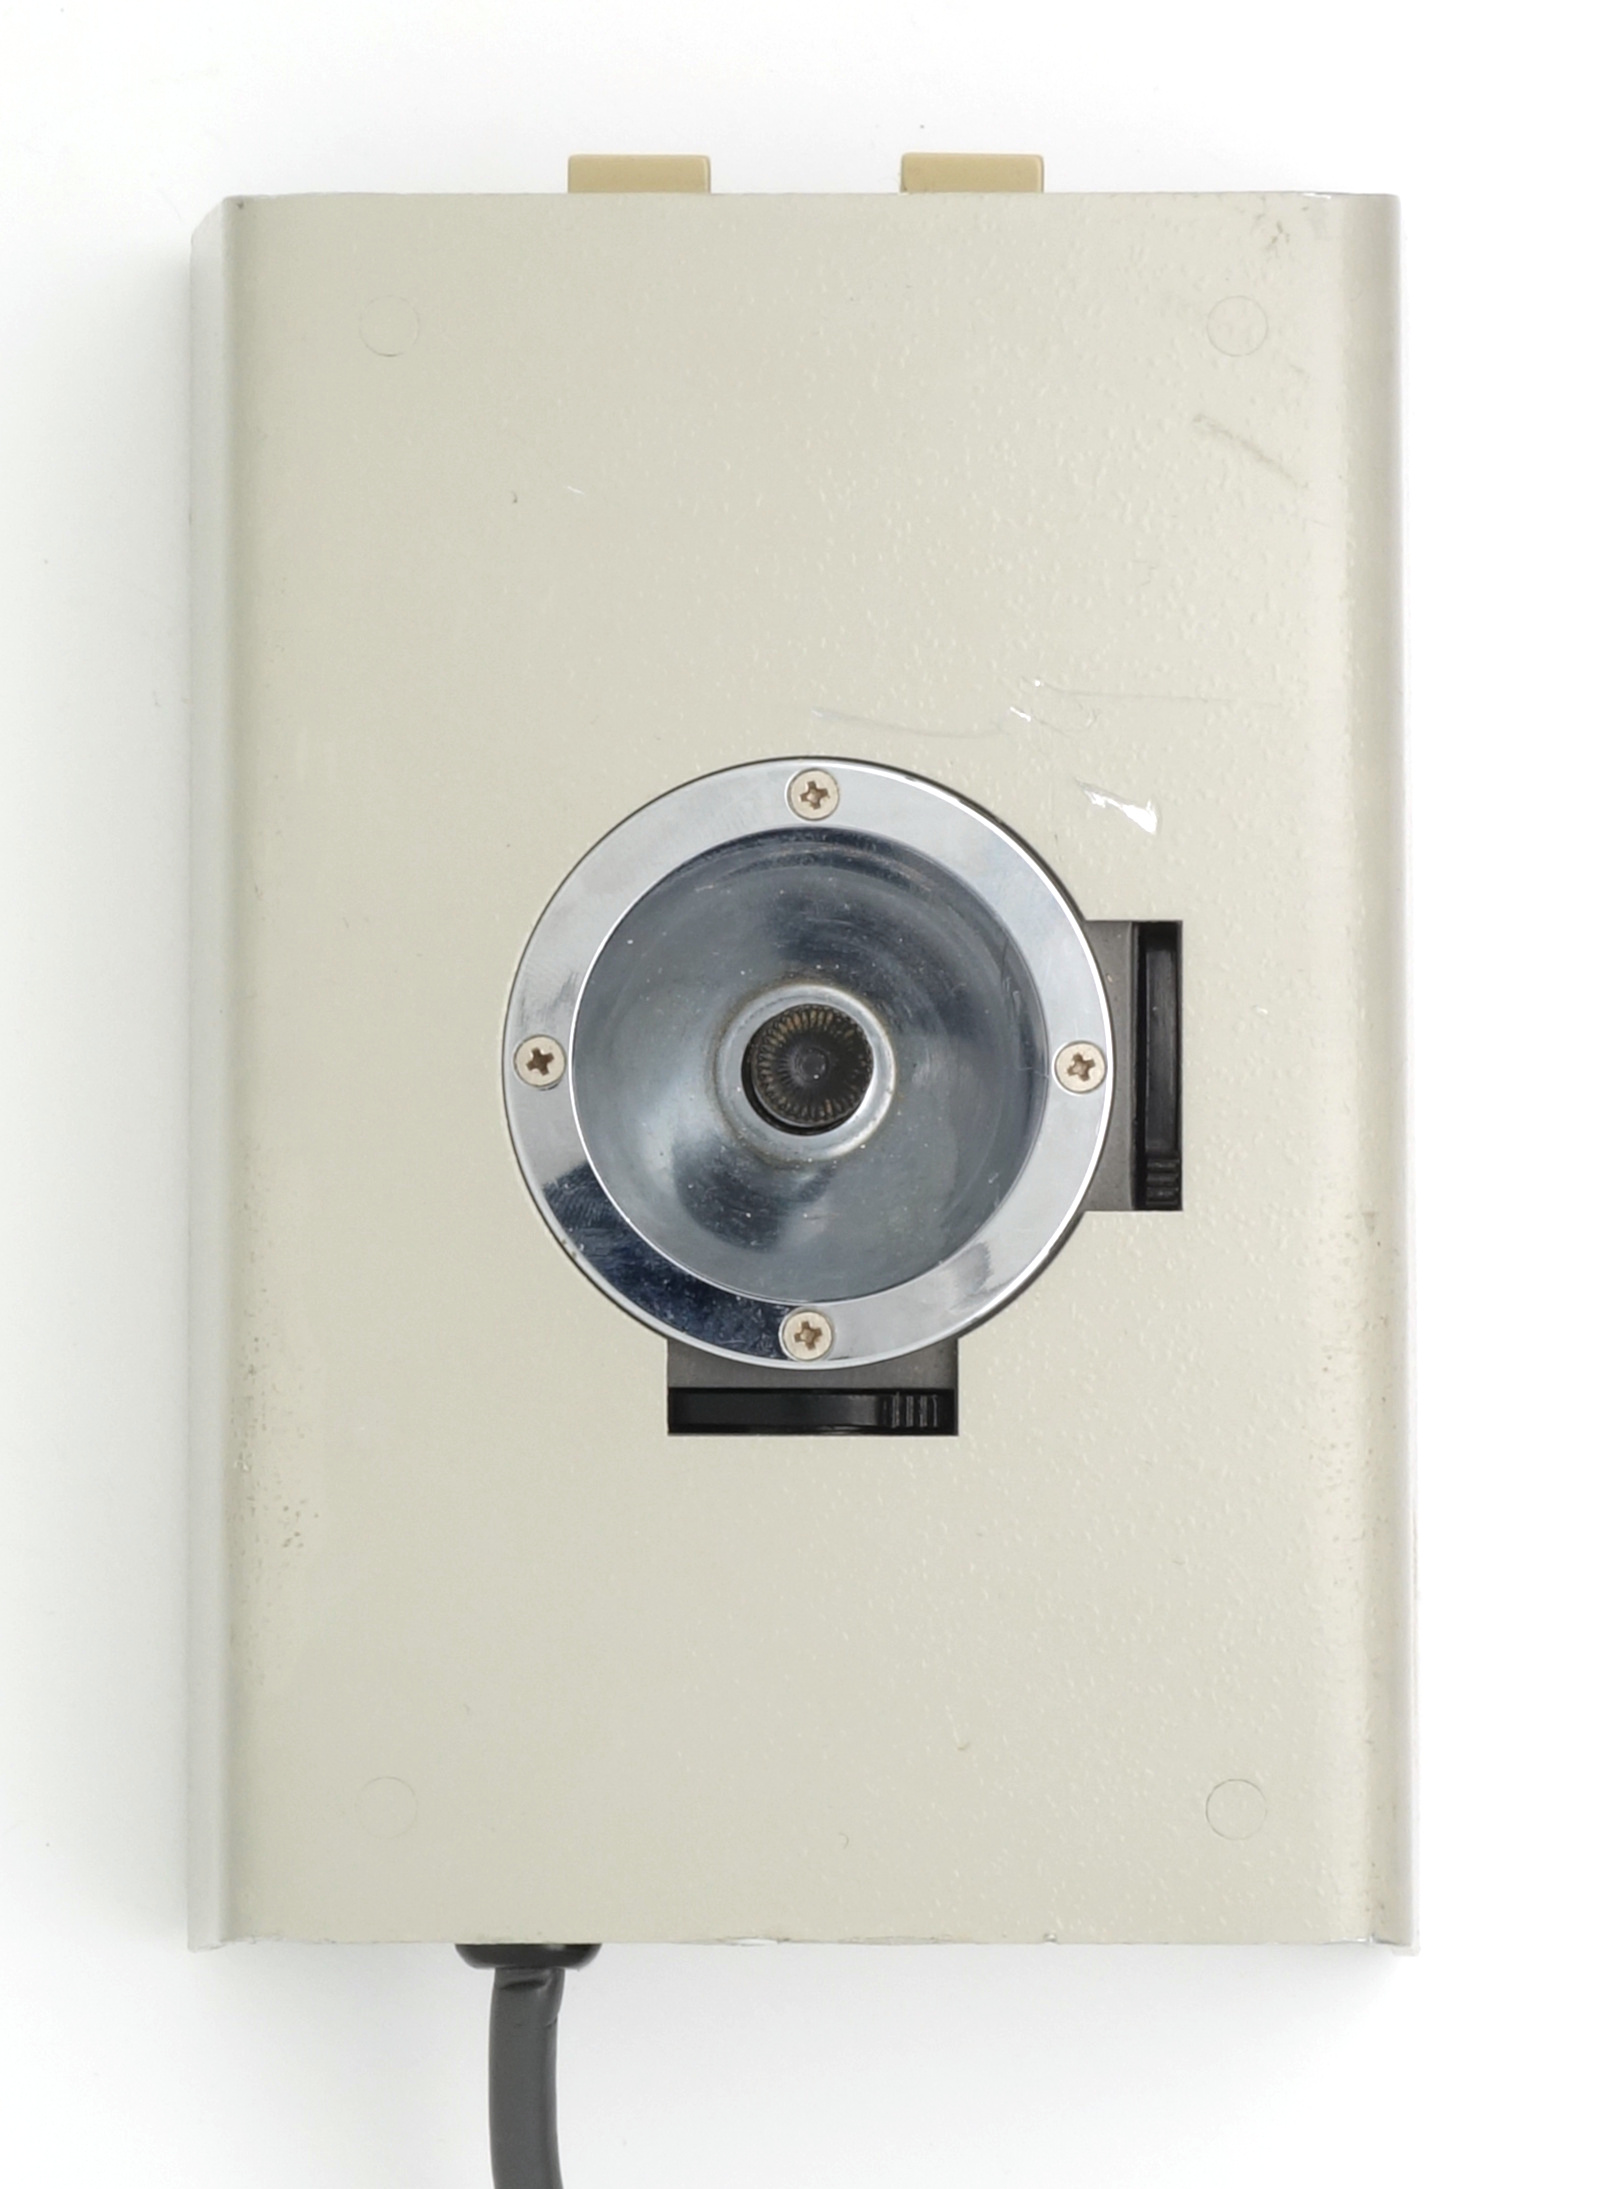
\includegraphics[scale=0.3]{1975_Tektronix_4952_Joystick/top_30.jpg}
    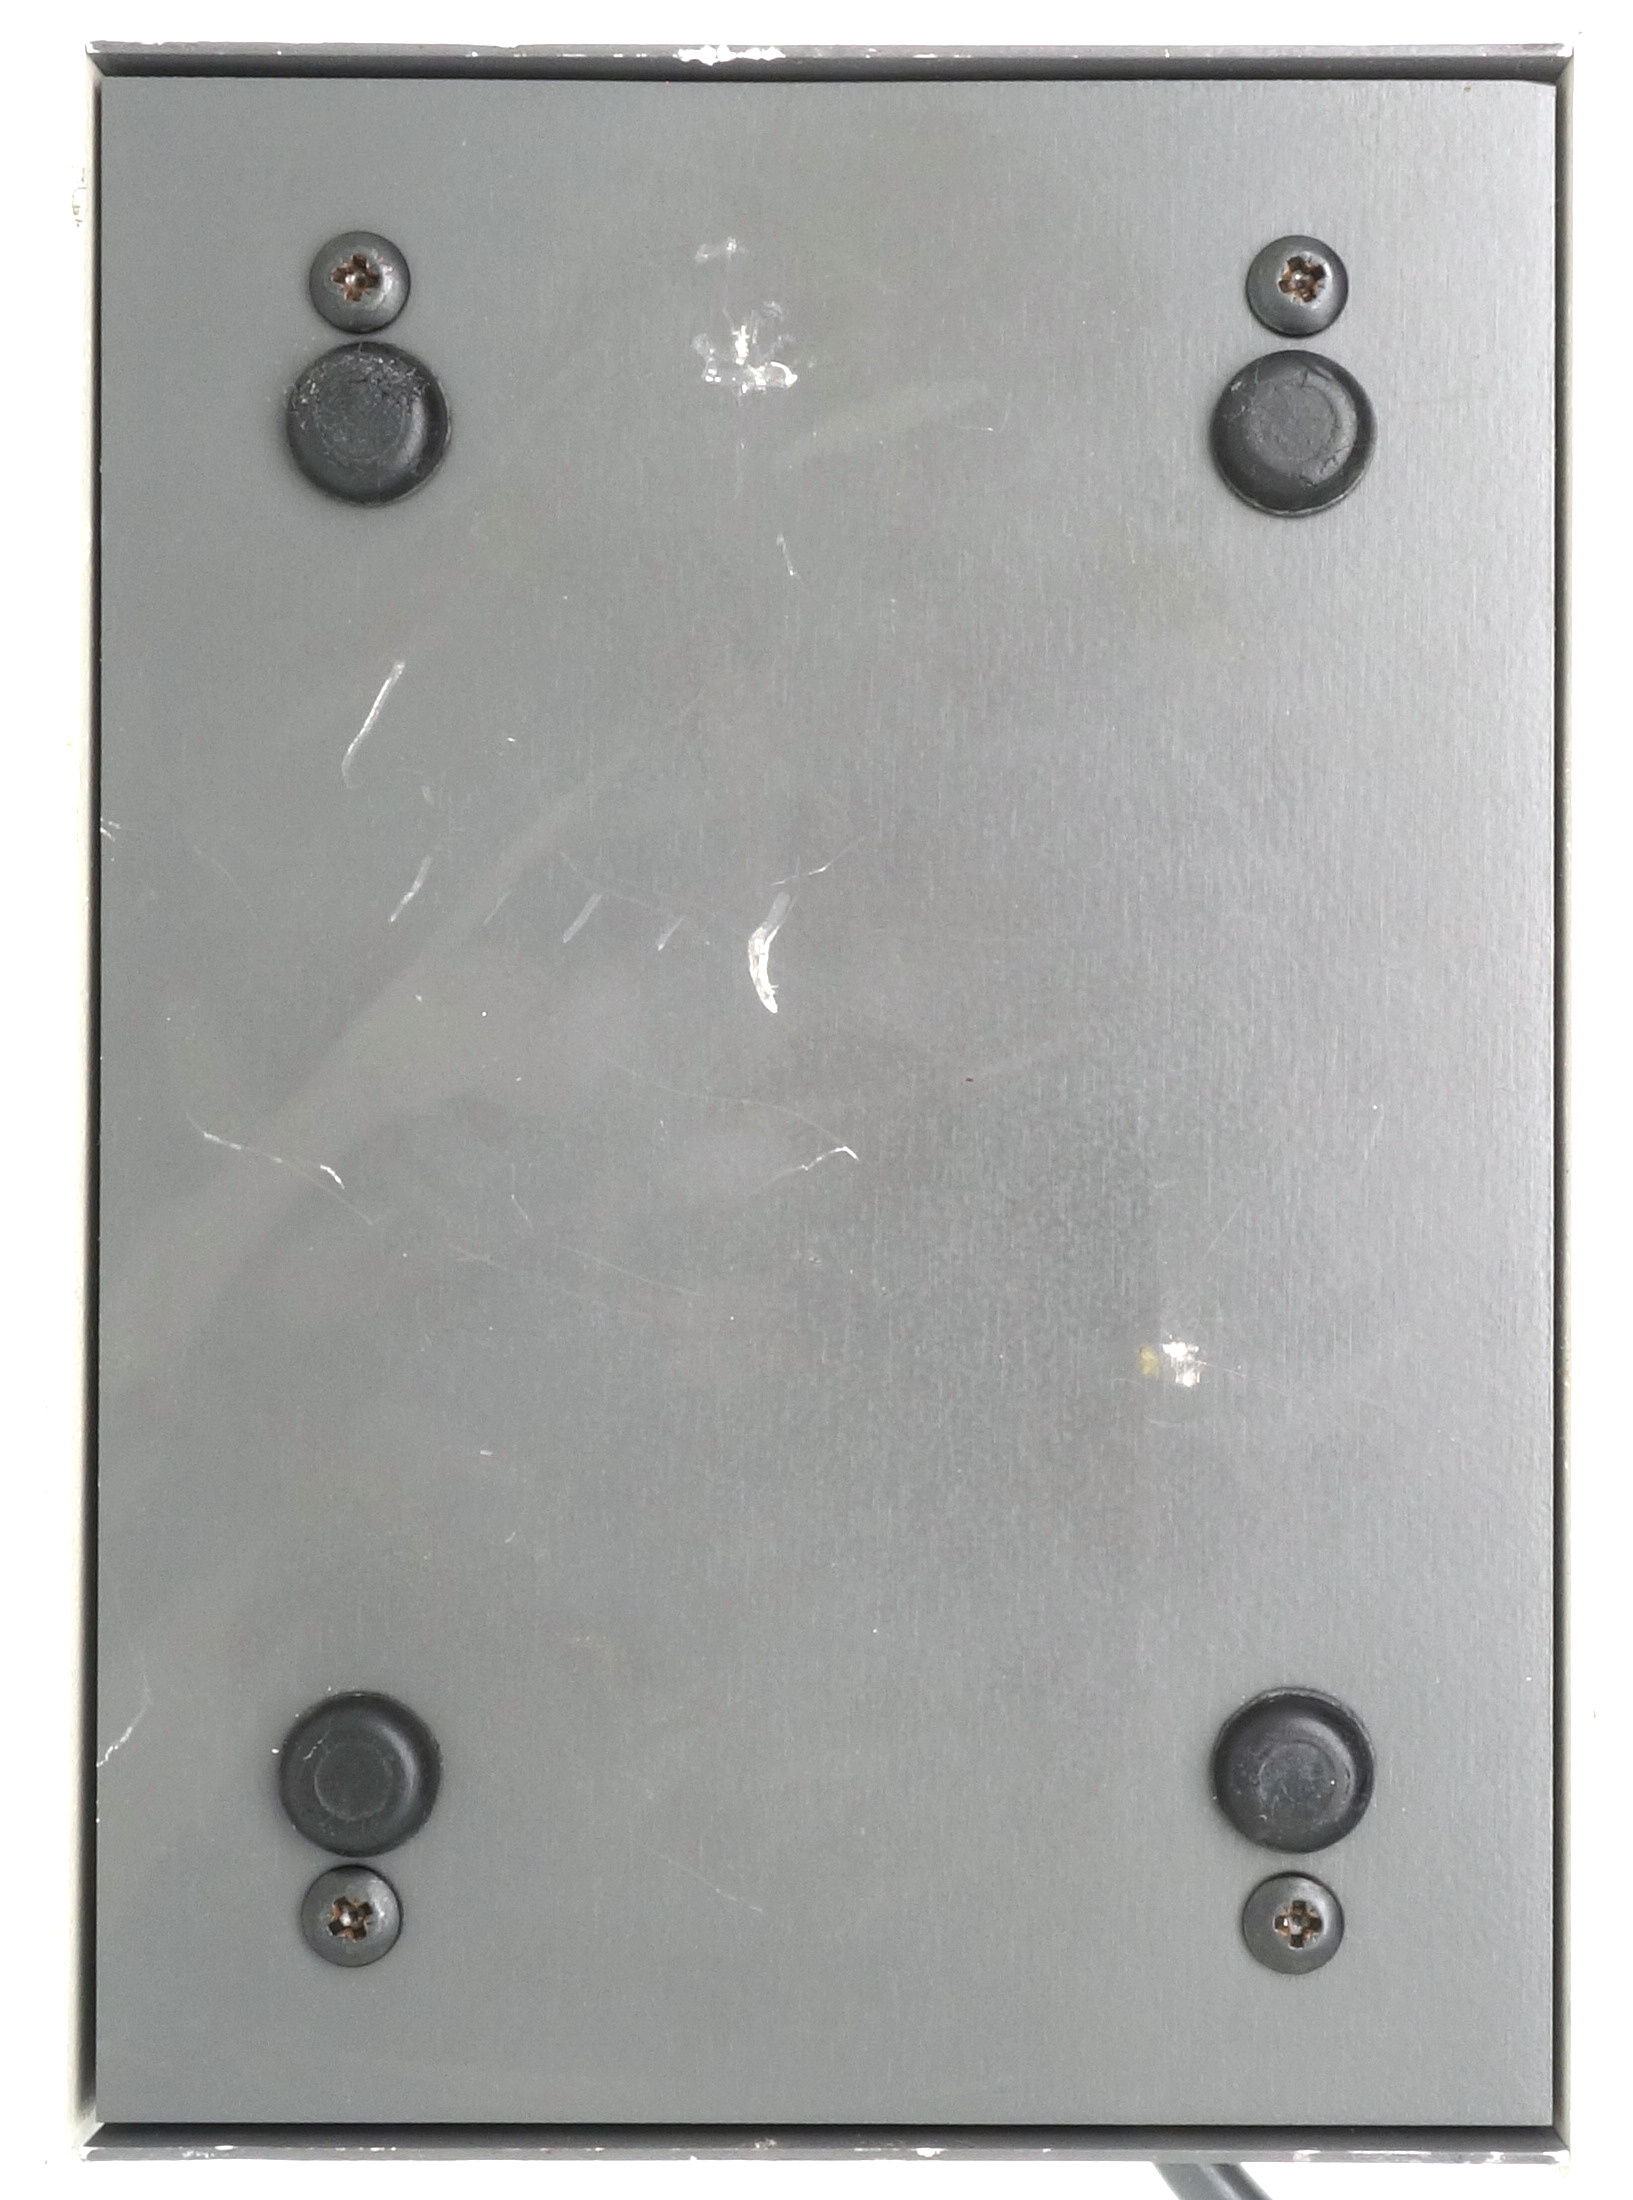
\includegraphics[scale=0.3]{1975_Tektronix_4952_Joystick/bottom_30.jpg}
    \caption{Джойстик Tektronix 4952 joystick, вид сверху и снизу}
    \label{fig:TektronixJoystickTopAndBottom}
\end{figure}

На лицевой стороне корпуса расположены две подписанные кнопки, а также название компании и модель устройства.
Корпус устройства весьма крупный (рис. \ref{fig:TektronixJoystickSize}).

\begin{figure}[h]
    \centering
    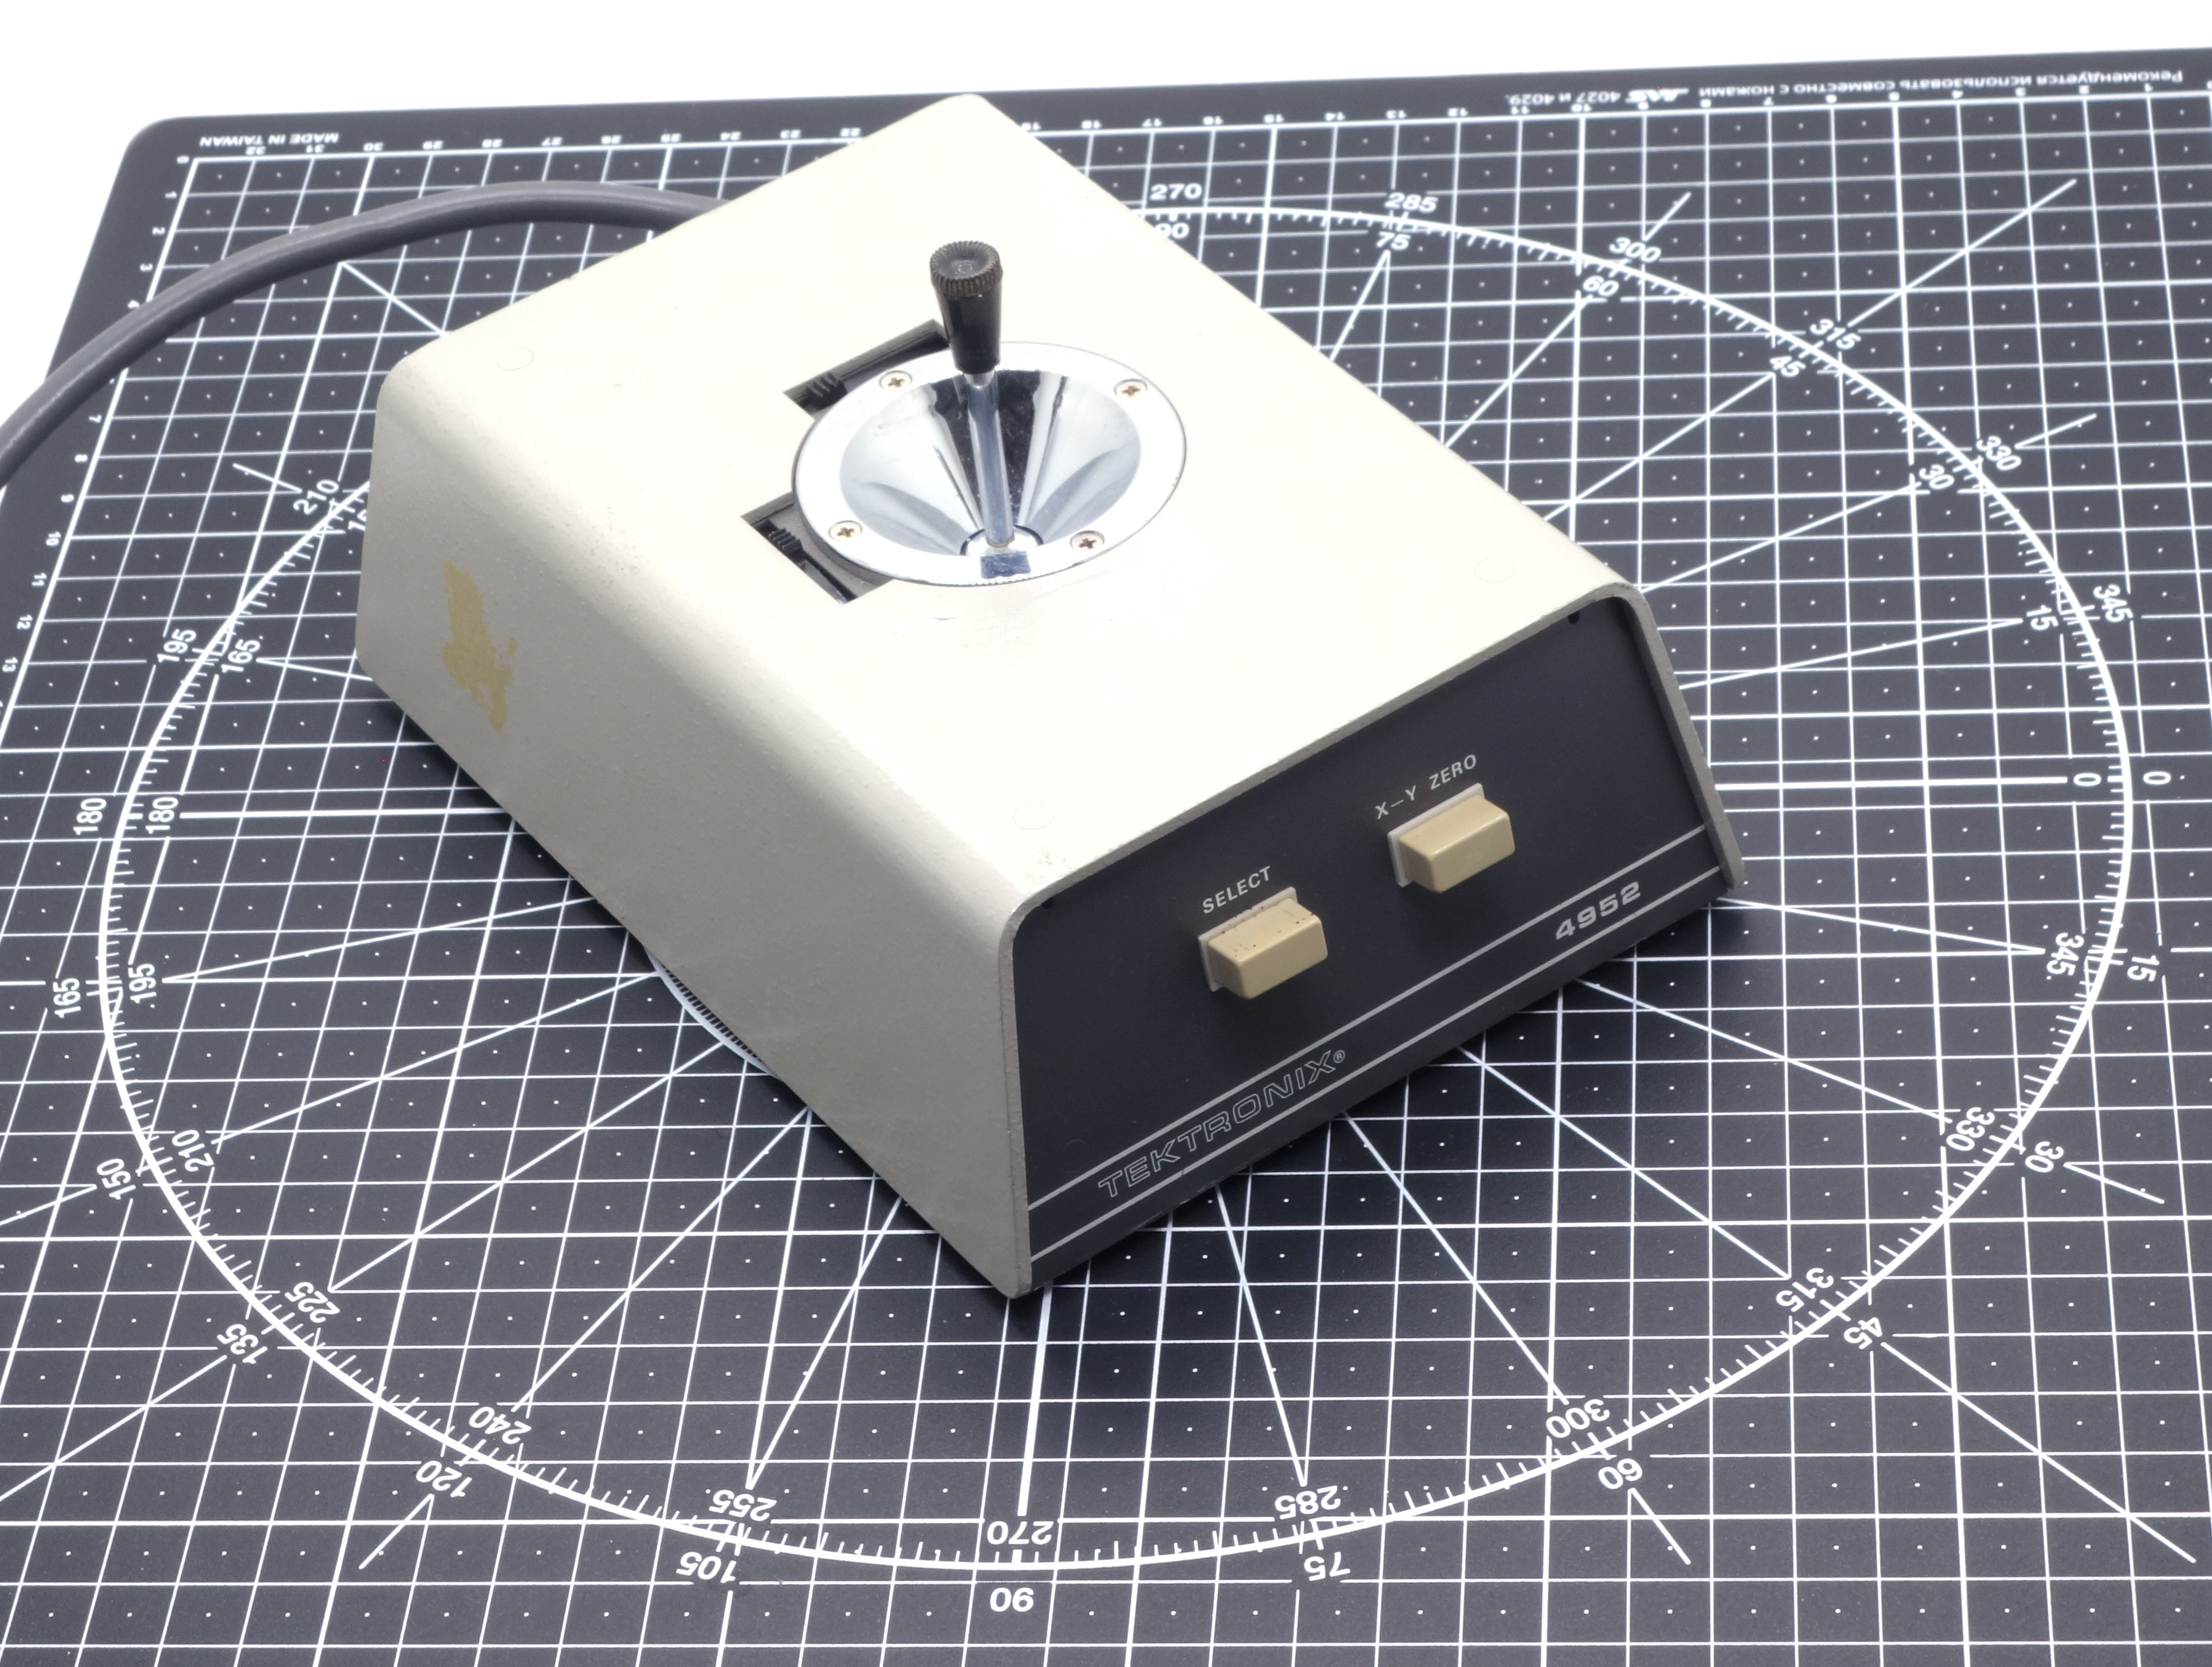
\includegraphics[scale=0.42]{1975_Tektronix_4952_Joystick/size_30.jpg}
    \caption{Джойстик Tektronix 4952 на размерном коврике с шагом сетки 1~см}
    \label{fig:TektronixJoystickSize}
\end{figure}

Рукоятку джойстика достаточно удобно двигать, обхватив пальцами и опираясь кистью на корпус. Размер корпуса не позволяет дотянуться до кнопок на передней панели, не убирая с него руку (рис. \ref{fig:TektronixJoystickHand}). Тем не менее, это было проблемой с учетом специфики использования устройства.

\begin{figure}[h]
    \centering
    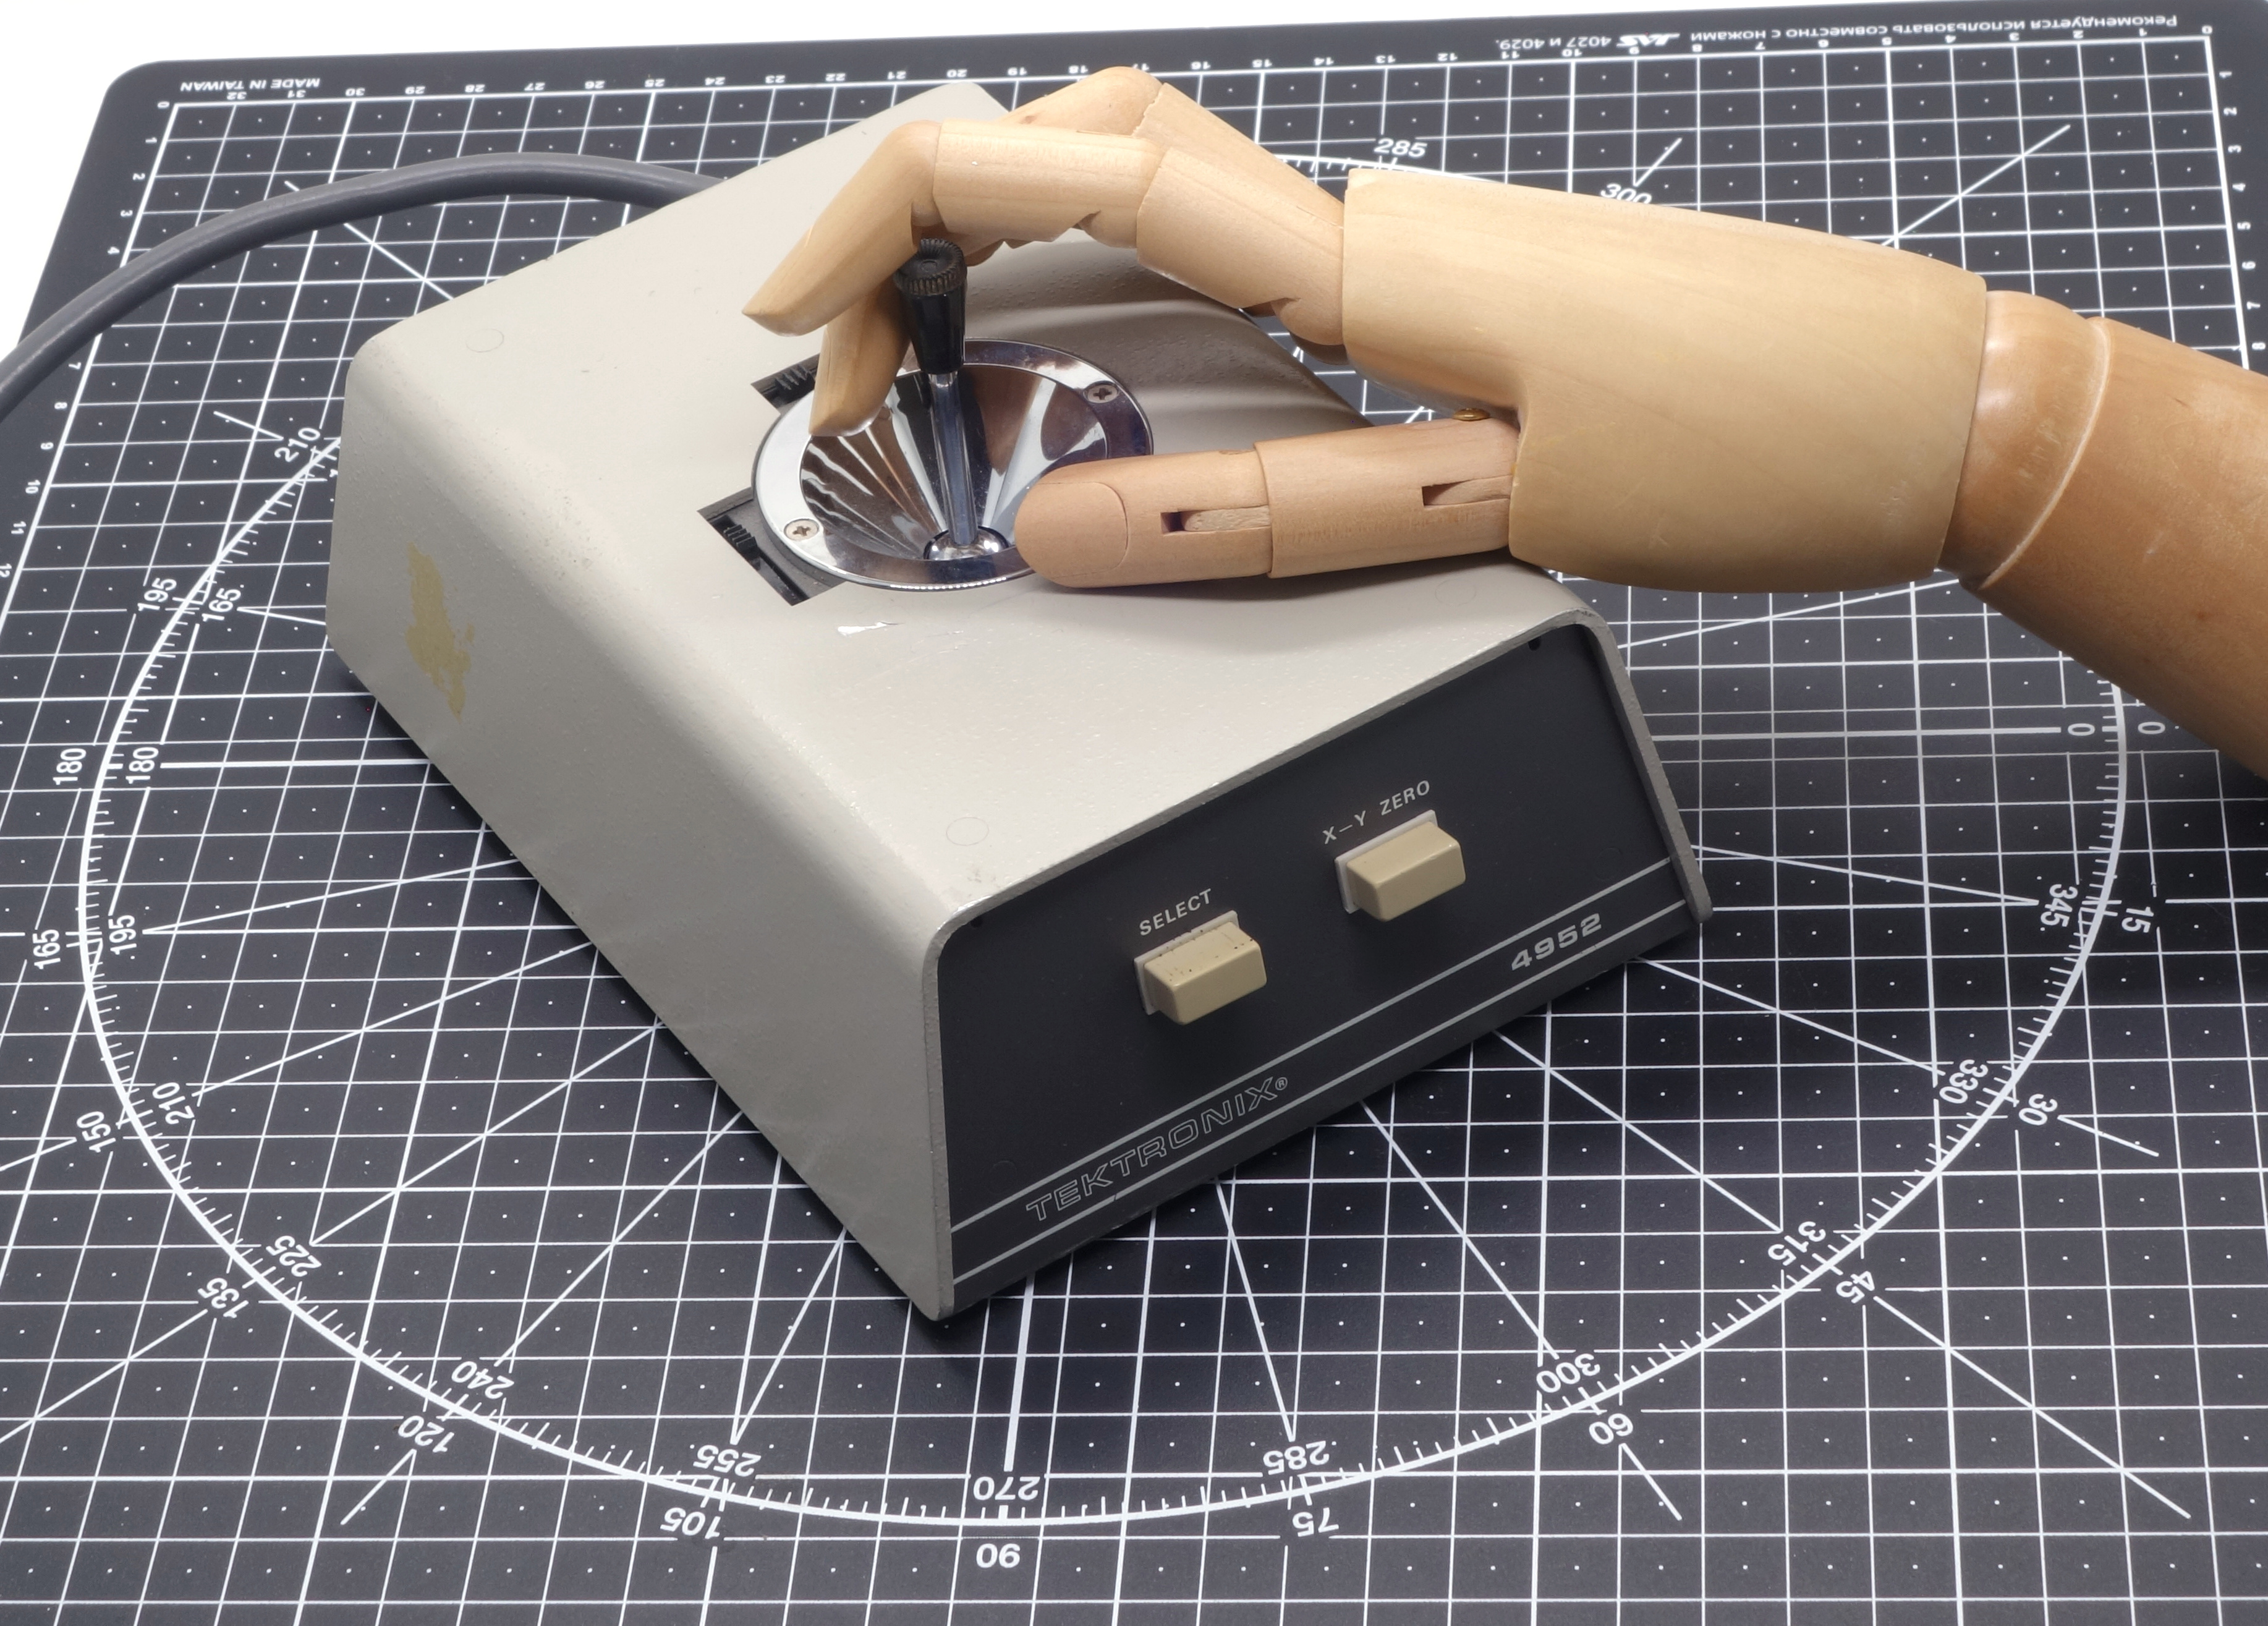
\includegraphics[scale=0.42]{1975_Tektronix_4952_Joystick/hand_05.jpg}
    \caption{Джойстик Tektronix 4952 с моделью руки человека}
    \label{fig:TektronixJoystickHand}
\end{figure}

\begin{itemize}
\item \verb!SELECT! это кнопка с фиксацией, необходимая только при использовании джойстика с графическими терминалами 4010: в зависимости от положения она позволяла перемещать <<перекрестие курсора>> (``cross-hair cursor'') либо с помощью джойстика, либо с помощью встроенных в терминал регуляторов колесного типа \cite{manual, manual2}. 

\item \verb!X-Y ZERO! это кнопка, нажатие на которую устанавливает на выходах джойстика $X$ и $Y$ нулевое напряжение, что приводит к немедленному перемещению курсора в центр экрана \cite{manual}.
\end{itemize}

Наклон рукоятки влияет на движение курсора предсказуемым образом: направление движения определяется направлением наклона, а угол наклона пропорционален скорости движения. Триммеры используются для регулировки дрейфа путем выставления нулевого напряжения на выходах $X$ и $Y$ при вертикальном положении рукоятки.

При работе пользователь смещает курсор к нужной точке на дисплее, отклоняя рукоятку джойстика, а затем программное обеспечение (например, система САПР) может получить в нужный момент координаты перекрестия курсора \cite{price}.

Джойстик подключался к системе с помощью длинного толстого кабеля. К компьютерам серии 4050 периферийные устройства подключались с помощью параллельной шины GPIB, а у терминалов 4010 был специальный адаптер, смонтированный в подставке терминала \cite{manual, manual2}.


В разобранном виде джойстик показан на рис. \ref{fig:TektronixJoystickInside}. 

\begin{figure}[h]
    \centering
    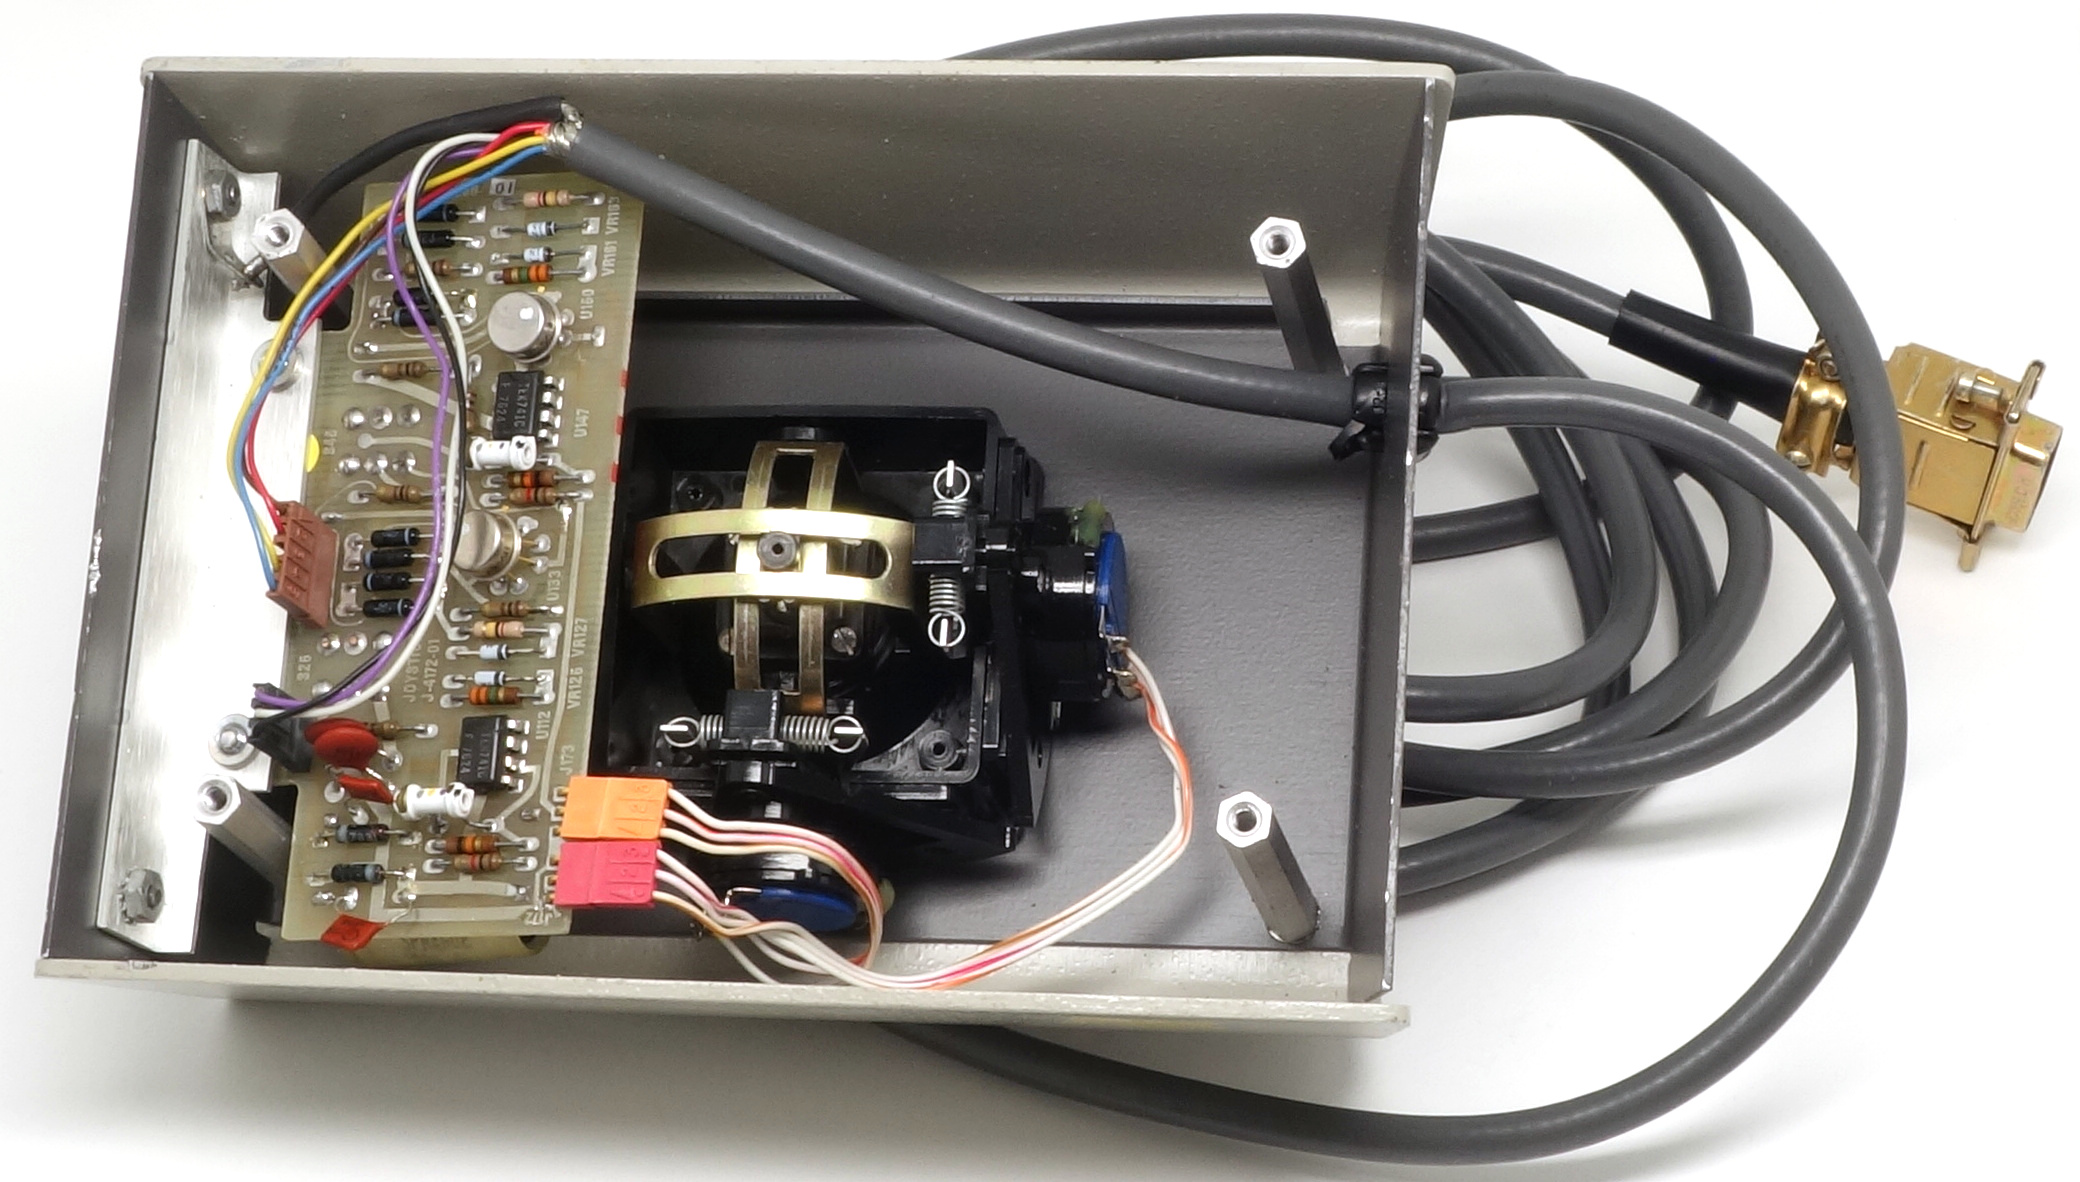
\includegraphics[scale=0.8]{1975_Tektronix_4952_Joystick/inside_30.jpg}
    \caption{Джойстик Tektronix 4952 в разобранном виде}
    \label{fig:TektronixJoystickInside}
\end{figure}

Смещение триммеров обеспечивает контроль дрейфа путем механического поворота потенциометров $X$ и $Y$. 

Сборный узел джойстика, включая стержень рукоятки и его крепление, а также потенциометры и конструкцию поворотных узлов корректировки дрейфа, является типовым: в дальнейшем он встречается в неизменном виде, вплоть до полной взаимозаменяемости, во многих аналоговых джойстиках, выпускаемых для промышленных нужд.

\begin{thebibliography}{9}
\bibitem {wiki} Tektronix 4050 -- Wikipedia \url{https://en.wikipedia.org/wiki/Tektronix_4050}
\bibitem {adv} Canadian Information Processing Society (CIPS) Computer Magazine - Vol. 5, Iss. 1-11, 1974. - p. 29
\bibitem {manual} TEKTRONIX 4952 JOYSTICK. Tektronix, Inc., JAN 1975. \url{http://www.bitsavers.org/pdf/tektronix/401x/070-1826-01_4952_Joystick_Jan75.pdf}
\bibitem {manual2} TEKTRONIX 4952 JOYSTICK OPTION 2. Instruction manual Tektronix, Inc., FEB 1976. \url{http://www.bitsavers.org/pdf/tektronix/405x/070-2098-00_4952_Joystick_Feb76.pdf}
\bibitem {price} Stanley J. Tektronix 4952 - Electronixandmore Vintage Electronics and Beyond. -- \url{https://electronixandmore.com/misc/index.php?item=56}
\end{thebibliography}
\end{document}
